\section{Parallel Performance}
\label{sec:parallel performance}
\todo{move to optimization section}
\subsection{Strong scaling - Amdahl's Law}
\label{sec:amdahls law}

Amdahl's Law approximates the potential speed up of a serial program.
The equation is presented in \cref{eq:amdahls law}, where $P$ is the portion of the serial code that can be parallelized, $(1-P)$ is the portion that cannot be parallelized and $n$ is the amount of processors available.
Thus, $S(n)$ is the theoretical speed up achievable while holding the workload constant.

\begin{equation}
  \label{eq:amdahls law}
  S(n) = \frac{1}{(1-P) + P/n}
\end{equation}

Amdahl's Law only applies if the amount of work performed in the parallel version is not significantly different than the serial code's amount of work.
An illustration of the potential speed up is presented in \cref{fig:amdahls law} with $n=1024$.
The model thus theorize that given a fully parallizable problem, the problem should be executed $n$ times faster~\cite{farber2011cuda}.

\begin{figure}[htb]
  \centering
  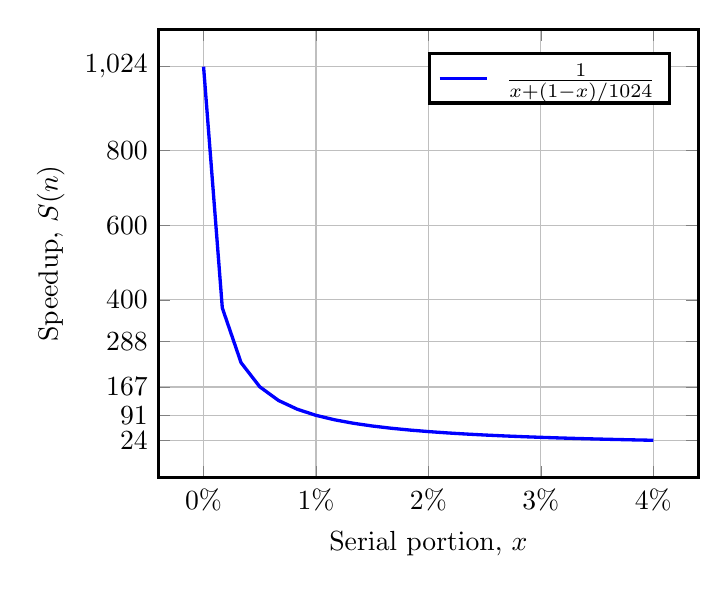
\begin{tikzpicture}
  \begin{axis}[
    ymajorgrids,
    xmajorgrids,
    ylabel={Speedup, $S(n)$},
    ytick={24,91,167,288,400,600,800,1024},
    xlabel={Serial portion, $x$},
    scaled x ticks = false, % do not add axis-multiplier
    xticklabel={% print percent
      \pgfmathparse{\tick*100}%
      \pgfmathprintnumber{\pgfmathresult}%
      \%%
    },
    legend style={
      at={(0.95,0.95)},
      anchor=north east,
      column sep=1ex
     },
     no markers,
     very thick
  ]

  \addplot+[domain=0.00:0.04] {1/(x+((1-x)/1024))};
  \addlegendentry{$\frac{1}{x + (1-x) / 1024}$};
  \end{axis}
\end{tikzpicture}

  \caption{Speed up by Amdahl's Law, where $x=(1-P)$, $(1-x)=P$, and $n=1024$}
  \label{fig:amdahls law}
\end{figure}

An important property of Amdahls is the decline of the curve as the solution moves from 0\% to 1\%.
With parallel portion $P=0.99$ the speed up is approximately $91\times$, and $1024\times$ when $P=1.00$ and everything can be executed in parallel.
According to Amdahl's Law, with just a tiny portion of the code that cannot be executed in parallel, a high speed up is not likely to be achieved.

\subsection{Gustafson-Barsis Law}
\label{sec:gustafson-barsis law}

Gustafson and Barsis Law approximates how much more throughput can be achieved by increasing processor count given a constant amount of time.
This type of formulation is often interesting when computing problems that are open ended such as computing pi -- given more computational power, the processors can compute more digits of pi in the same time~\cite{amdahlorgustafson2011}.

\begin{equation}
  \label{eq:gustafson-barsis law}
  W(n) = n + (1-n) \times (1-P)
\end{equation}
Where $P$ is the amount of the program that can be parallelized and $W(n)$ is the theoretical increase in throughput over a defined period of time.~\cite{gustafson1988reevaluating}.

